\newpage

\section{Návrh}

Na základe analýzy problémovej oblasti a existujúcich riešení sme sa rozhodli najprv použiť konvolučnú neurónovú sieť (jej popis a architektúra v kapitole \ref{nn_popis}), čo sa pretavilo aj do prvotných experimentov (kapitola \ref{first_experiments}) vykonávaných v rámci predmetu Počítačové videnie\footnote{http://vgg.fiit.stuba.sk/teaching/computer-vision/}.

\subsection{Návrh neurónovej siete}
\label{nn_popis}
\iffalse
K predikcii pohľadov na webové stránky je vhodné použiť konvolučnú neurónovú sieť, keďže webstránky sú vo forme obrázkov. Neurónová sieť bude predikovať priamo výslednú teplotnú mapu pohľadov (mapu výraznosti). Sieť by mala pozostávať z konvolučnej a združovacej vrstvy (vrstiev) pre spracovanie obrázku, nasledovaných normalizačnou vrstvou, plne prepojenou vrstvou a vrstvou výpadku (z angl. dropout layer). Za nimi nasleduje už len výstupná vrstva. Ako aktivačnú funkciu sme vybrali sigmoid, nakoľko sa bude predikovať mapa výraznosti, t. j. v podstate pravdepodobnosť pohľadu. 
\fi 
Celá architektúra je načrtnutá na schéme na obrázku \ref{my_tensorboard_cnn} vytvorenej pomocou nástroja  TensorBoard\footnote{https://www.tensorflow.org/get\_started/summaries\_and\_tensorboard/}.


\begin{figure}[H]
	\begin{center}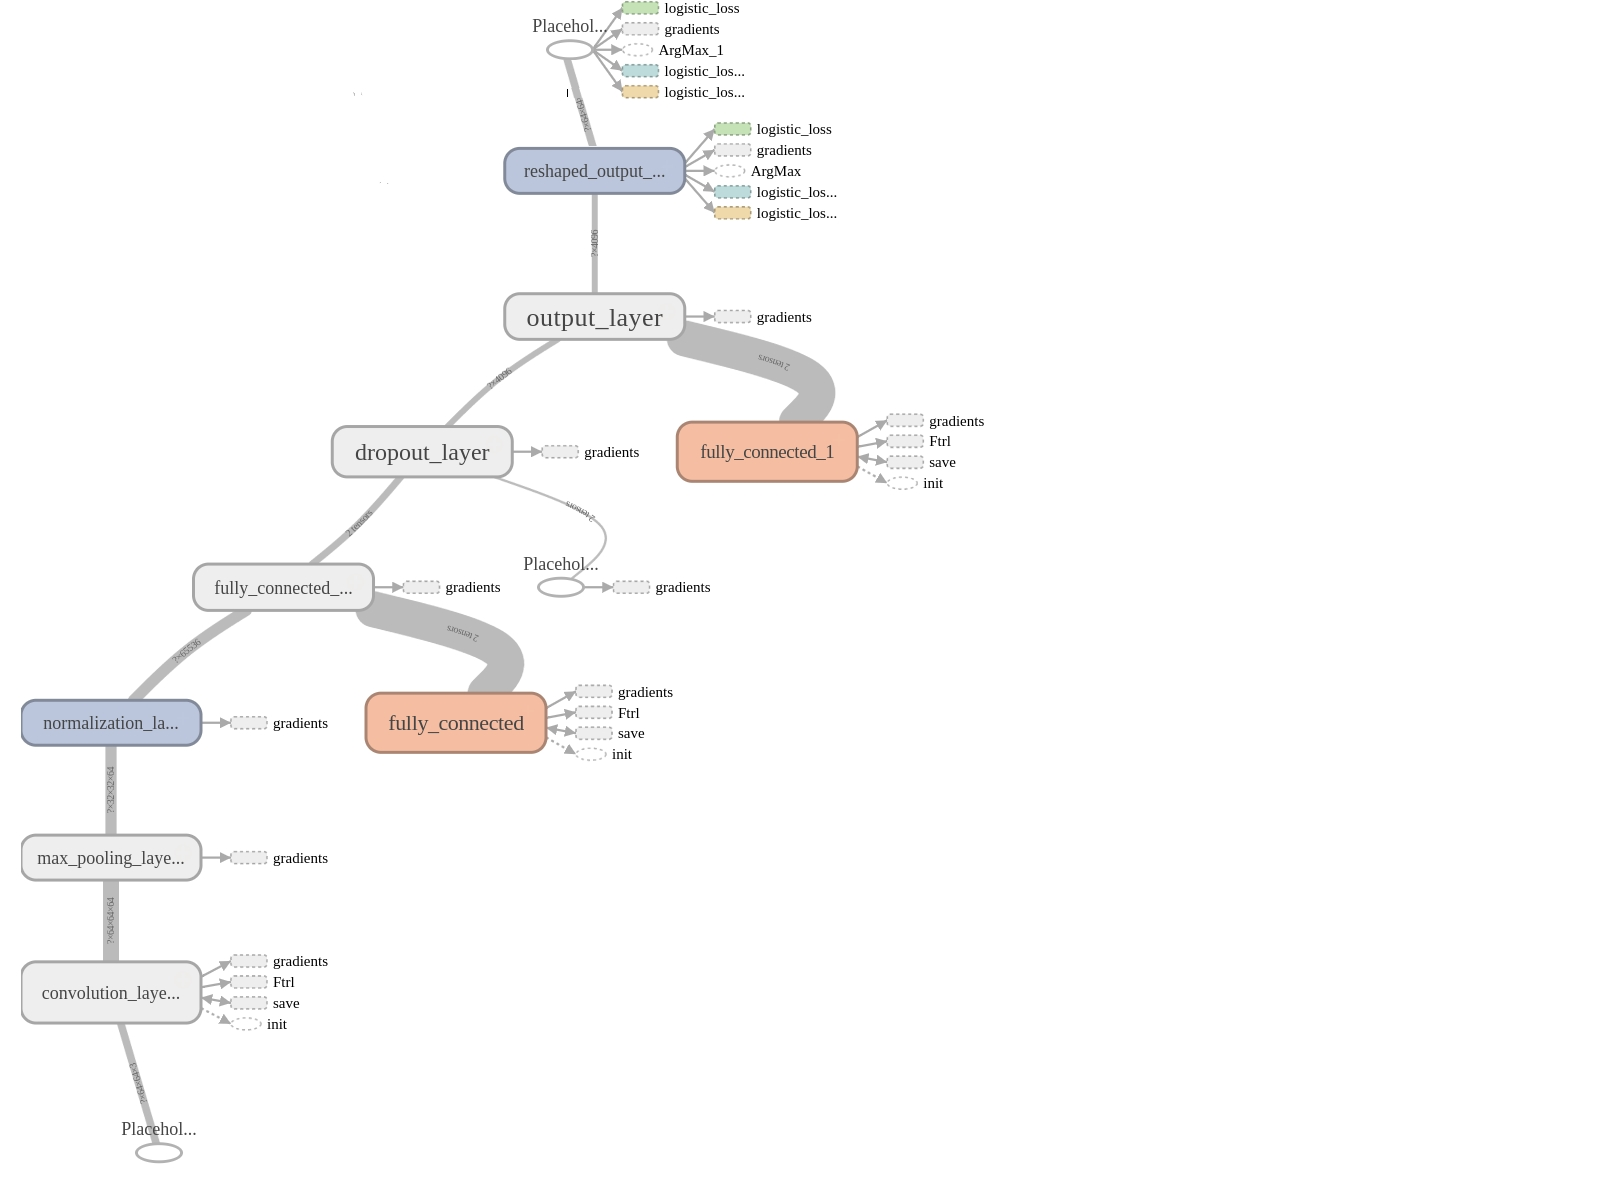
\includegraphics[scale=0.4]{graph-run.jpg}
		\caption[Návrh neurónovej siete]{
			Grafická schéma neurónovej siete, zdola vstup, vrstvy neurónovej siete, výstup (predikovaná mapa výraznosti)
		}\label{my_tensorboard_cnn}
	\end{center}
\end{figure}
\iffalse
Na konvolučnej vrstve sa použije konvolučný filter o veľkosti 5x5, ktorým sa prejde vstupný obrázok. Výstupom z nej budú mapy (obrázky) po aplikovaní filtra. Tieto dáta budú spracovávané vo vrstve združovania s použitím operácie MAX, okna (filtra) s veľkosťou 2x2 a posunom s veľkosťou 2. Výstup všetkých filtrov je zlúčený do jednej širokej vrstvy a to normalizačnej. Z nej nasledujú prepojenia do plne prepojenej vrstvy, za ktorou nasleduje vrstva výpadku\cite{dropout}. Tá prakticky obsahuje hodnotu (od 0 do 1) určujúcu koľko neurónov bude dočasne „odstránených“ z modelu spolu so všetkými spojeniami, ako vstupnými tak aj výstupnými. To by malo zabrániť pretrénovaniu siete. Za vrstvou výpadku nasleduje už len výstupná vrstva, ktorá je nakoniec ešte aj transformovaná do 2D matice reprezentujúcej predikovanú mapu výraznosti. 

Aktivačná funkcia sigmoid bude použitá iba na prvej konvolučnej vrstve a na plne prepojenej vrstve. K trénovaniu sa použije FTRL optimizér spolu s náhodným generátorom dát, ktorý bude z datasetu určenému pre fázu trénovania náhodne vyberať dáta na učenie. Tým sa zabezpečí simulácia náhodnosti vstupných dát a teda sa sieť bude schopná lepšie učiť. 
\fi 

\subsection{Prvotné experimenty}
\label{first_experiments}

\subsection{Dataset}
\label{dataset}


\iffalse
\begin{equation}
content...
\end{equation}
\fi